\documentclass[a4paper]{article}

\usepackage[margin=2cm]{geometry}		% For desired margins
\usepackage{fontspec}					% utf-8 support
\usepackage{enumitem}					% Continuous enumerations
\usepackage{float}						% Floating images
\usepackage[dvipsnames]{xcolor}			% Colors
\usepackage{pgfplots}					% Custom plots
\usepackage{listings}					% Code highlighting
\usepackage[hidelinks]{hyperref}		% Hyper links
\usepackage{graphicx}					% To include images
\usepackage{tikz}						% To draw images
\usepackage{pgfplots}					% To draw graphs
\usepackage[dvipsnames]{xcolor	}
\usepackage{subcaption}

\pgfplotsset{compat=1.13}
\usetikzlibrary{positioning}

\setlength{\parindent}{0pt}
\setlength{\parskip}{1em}

\title{PAR: Laboratory 5 \\
		\texttt{\large par4201}}
\author{Joan Marcè i Igual \and Es6teve Tarragó i Sanchis}

\newenvironment{questionenum}{%
\setlist[enumerate]{resume}
\restartlist{enumerate}
\newcommand{\question}[1]{
\begin{enumerate}
	\item\bfseries ##1
\end{enumerate}
}}{%
}

\lstset{
	basicstyle=\small\ttfamily,
	showspaces=false,
	showstringspaces=false,
	tabsize=4,
	numbers=left,
	numbersep=5pt,
	stringstyle=\color{orange},
	commentstyle=\color{OliveGreen},
	keywordstyle=\color{blue},
	numberstyle=\color{Gray},
	frame=single
}

\begin{document}
\maketitle
\tableofcontents

\section{Analysis with Tareador}

\begin{questionenum}
	\question{Include the relevant parts of the modified \texttt{solver-tareador.c} code and comment where the calls to the Tareador API have been placed. Comment also about the task graph generated and the causes of the dependencies that appear in the two solvers: \emph{Jacobi} and \emph{Gauss-Seidel}. How will you protect them in the parallel \texttt{OpenMP} code.}
\end{questionenum}

\begin{center}	
	\begin{minipage}{0.8\textwidth}
\begin{lstlisting}[language=C, title=\texttt{heat-tareador.c}]
switch( param.algorithm ) {
	case 0: // JACOBI
		tareador_start_task("relax_jacobi");
		residual = relax_jacobi(param.u, param.uhelp, np, np);
		tareador_end_task("relax_jacobi");
		// Copy uhelp into u
		tareador_start_task("Copy_mat");
		copy_mat(param.uhelp, param.u, np, np);
		tareador_end_task("Copy_mat");
		break;
	case 1: // GAUSS
		tareador_start_task("relax_gauss");
		residual = relax_gauss(param.u, np, np);
		tareador_end_task("relax_gauss");
		break;
}
		\end{lstlisting}
	\end{minipage}
	
	\begin{minipage}{0.8\textwidth}
		\begin{lstlisting}[language=C, title=\texttt{solver-tareador.c}]
// Set tareador task
tareador_start_task("jacobi_relax");
// Disable sum object for better parallelization potential
tareador_disable_object(&sum);
utmp[i*sizey+j]= 0.25 * ( u[ i*sizey     + (j-1) ]+  // left
u[ i*sizey     + (j+1) ]+  // right
u[ (i-1)*sizey + j     ]+  // top
u[ (i+1)*sizey + j     ]); // bottom
diff = utmp[i*sizey+j] - u[i*sizey + j];
sum += diff * diff;

// Reenable sum object
tareador_enable_object(&u);

// End of tareador task
tareador_end_task("jacobi_relax");
		\end{lstlisting}
	\end{minipage}
\end{center}

\section{OpenMP parallelization and execution analysis: \emph{Jacobi}}
\begin{questionenum}
	\question{Describe the data decomposition strategy that is applied to solve the problem, including a picture with the part of the data structure that is assigned to each processor.}
	
	The decomposition strategy used is giving each thread a different part of the matrix by rows. This can be seen in the \autoref{fig:jacobi-data} where each thread has a different block of rows of the matrix to be computed. 
	
	\begin{figure}[H]
		\centering
		
\includegraphics[width=0.5\textwidth]{images/jacobi/data}
		\caption{Figure describing the data decomposition, each thread has one color}
		\label{fig:jacobi-data}
	\end{figure}
	
	\question{Include the relevant portions of the parallel code that you implemented to solve the heat equation using the \emph{Jacobi} solver, commenting whatever necessary. Including captures of Paraver windows to justify your explanations and the differences observed in the execution.}
	
	The heat computation part can be optimized in the following way with \texttt{OpenMP}. 
	\begin{center}
		
	\begin{minipage}{0.9\textwidth}
		\begin{lstlisting}[language=C, title=\texttt{solver-tareador.c}]
double relax_jacobi (double *u, double *utmp, unsigned sizex, unsigned sizey)
{
	double diff, sum=0.0;
	
	// In this part max threads is used instead of get_num_threads() beacuse 
	// there's only one thread at this point.
	int howmany = omp_get_max_threads();
		
	// Parallelize by blocks, assigning each block to one different thread
	#pragma omp parallel for reduction(+:sum) private(diff)
	for (int blockid = 0; blockid < howmany; ++blockid) {
		int i_start = lowerb(blockid, howmany, sizex);
		int i_end = upperb(blockid, howmany, sizex);
		for (int i=max(1, i_start); i<= min(sizex-2, i_end); i++) {
			for (int j=1; j<= sizey-2; j++) {
				utmp[i*sizey+j]= 0.25 * ( u[ i*sizey     + (j-1) ]+  // left
				u[ i*sizey     + (j+1) ]+  // right
				u[ (i-1)*sizey + j     ]+  // top
				u[ (i+1)*sizey + j     ]); // bottom
				diff = utmp[i*sizey+j] - u[i*sizey + j];
				sum += diff * diff;
			}
		}
	}
	
	return sum;
}
		\end{lstlisting}
	\end{minipage}
	\end{center}
	
	Also there's another complementary way to optimize. The \texttt{copy\_mat()} function can be parallelized to allow a better way of copying the matrix.
	
	\begin{center}
		\begin{minipage}{0.8\textwidth}
			\begin{lstlisting}[language=C, title=\texttt{solver-tareador.c}]
#pragma omp parallel for collapse(2)
for (int i=1; i<=sizex-2; i++)
	for (int j=1; j<=sizey-2; j++)
		v[ i*sizey+j] = u[ i*sizey+j ];
			\end{lstlisting}
		\end{minipage}
	\end{center}

	Another way to attack the problem is avoiding the matrix copy part and only swapping the pointers of the matrix. This can be done in the \texttt{heat-omp.c} file between the iterations.
	
	\begin{center}
		\begin{minipage}{0.8\textwidth}
			\begin{lstlisting}[language=C, title=\texttt{heat-omp.c}]
residual = relax_jacobi(param.u, param.uhelp, np, np);
// Swap the pointers to avoid copying the matrix
double *temp = param.u;
param.u = param.uhelp;
param.uhelp = temp;

// Disable the matrix copy
//copy_mat(param.uhelp, param.u, np, np);
			\end{lstlisting}
		\end{minipage}
	\end{center}
	
	\begin{figure}[H]
		\centering
		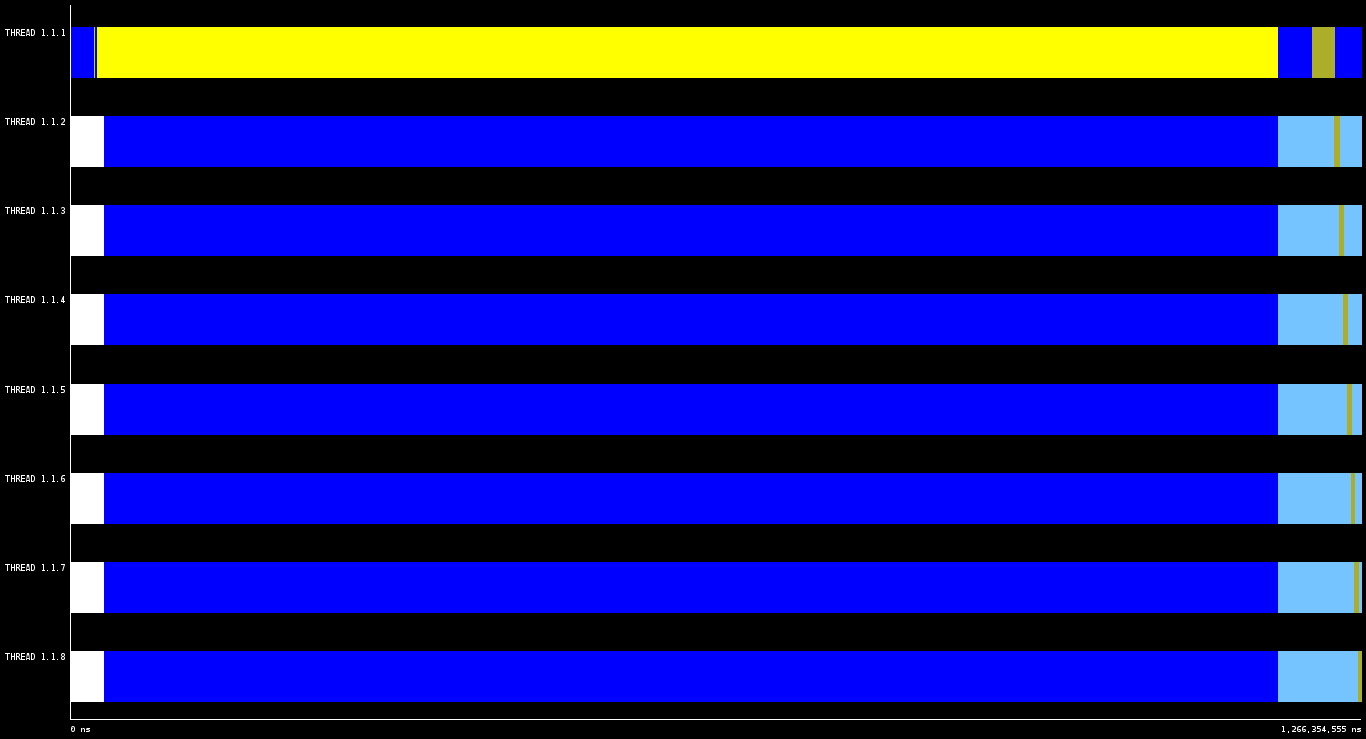
\includegraphics[width=\textwidth]{images/jacobi/paraver-8}
		\caption{Capture of \texttt{paraver} using 8 processors}
		\label{fig:jacobi-paraver}
	\end{figure}

	\begin{figure}[H]
		\centering
		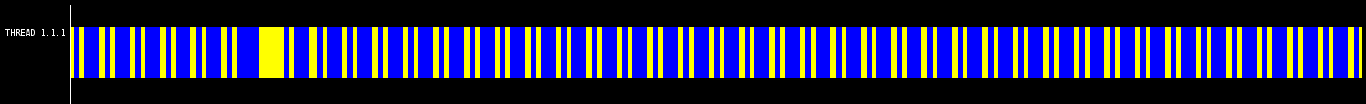
\includegraphics[width=\textwidth]{images/jacobi/paraver-8-zoom}
		\caption{Zoom of \texttt{paraver} capture to show that the processor 0 is still doing work}
		\label{fig:jacobi-paraver-zoom}
	\end{figure}
	
	As it can be seen in the \autoref{fig:jacobi-paraver} all processors are working so the work is properly shared between all the processors. It seems that the processor 0 is only doing synchronizations but actually it's working too as it can be seen in the \autoref{fig:jacobi-paraver-zoom}.
	
	\question{Include the speed-up (strong scalability) plots that have been obtained for the different numbers of processors. Reason about the performance that is observed.}
	
	\begin{figure}[H]
		\begin{subfigure}[t]{0.49\textwidth}
			\begin{tikzpicture}
				\begin{axis}[
						width = \textwidth,
						xmin = 1, xmax = 12,
						domain = 0:12,
						xlabel = number of processors,
						ylabel = execution time,
						enlarge x limits = 0.05,
					]
					\addplot table[x = P, y = T]{data/jacobi/elapsed.csv};
					\addplot[dashed, mark = none] {4.5/x};
				\end{axis}
			\end{tikzpicture}
			\caption{Elapsed time for each number of processors}
			\label{fig:jacobi-elapsed}
		\end{subfigure}
		\hfill
		\begin{subfigure}[t]{0.49\textwidth}		
			\begin{tikzpicture}
				\begin{axis}[
						width = \textwidth,
						xmin = 1, xmax = 12,
						ymin = 0, ymax = 12,
						domain = 0:12,
						xlabel = number of processors,
						ylabel = speedup,
						enlarge x limits = 0.05,
					]
					\addplot[dashed, mark=none]{x};
					\addplot table[x = P, y = S]{data/jacobi/speedup.csv};
				\end{axis}
			\end{tikzpicture}
			\caption{Speedup obtained for each number of processors}
			\label{fig:jacobi-speedup}
		\end{subfigure}
	\caption{Comparison between speedup and elapsed time by number of processors in the Jacobi solution}
	\end{figure}
\end{questionenum}

As it can bee seen in the \autoref{fig:jacobi-speedup} the speedup increases and then it remains nearly constant. This is due to the overhead caused by \texttt{OpenMP} as the number of processors increases. If the data is divided by many processors there's more time spend during the synchronization than computing the value and that's why the speedup is not increasing anymore.

\section{OpenMP parallelization and the execution analysis: \emph{Gauss-Seidel}}
\begin{questionenum}
	\question{Include the relevant portions of the parallel code that implements the \emph{Gauss-Seidel} solver, commenting how you implemented the synchronization between threads.}
	
	\begin{center}
		\begin{minipage}{0.8\textwidth}
			\begin{lstlisting}[language=C, title=\texttt{solver-omp-gauss.c}]
double relax_gauss (double *u, unsigned sizex, unsigned sizey)
{    
	int howmany = omp_get_max_threads();
	int numblocks = howmany;
	int blocksfinished[numblocks];
	for(int i =0; i < numblocks; ++i) blocksfinished[i]=-1;
	double unew, diff, sum=0.0;
	
	#pragma omp parallel for reduction(+:sum) private(diff,unew)
	for (int blockid = 0; blockid < numblocks; ++blockid) {
		for (int blockidcol = 0; blockidcol < numblocks; ++blockidcol){
			if (blockid > 0) {
				// Added block waiting
				while( blocksfinished[blockid-1] < blockidcol ) {
				#pragma omp flush(blocksfinished)
			}
		}
		int i_start = lowerb(blockid, numblocks, sizex);
		int i_end = upperb(blockid, numblocks, sizex);
		int j_start = lowerb(blockidcol,numblocks, sizey);
		int j_end = upperb(blockidcol, numblocks,sizey);
		for (int i=max(1, i_start); i<= min(sizex-2, i_end); i++) {
			for (int j=max(1, j_start); j<= min(sizey-2, j_end); j++) {
				unew = 0.25 * (
					u[ i*sizey 		+ (j-1) ]+  // left
					u[ i*sizey		+ (j+1) ]+  // right
					u[ (i-1)*sizey	+ j     ]+  // top
					u[ (i+1)*sizey	+ j     ]); // bottom
				diff = unew - u[i*sizey+ j];
				sum += diff * diff;
				u[i*sizey+j]=unew;
				}
			}
			
			// Finish block
			blocksfinished[blockid] = blockidcol;
			#pragma omp flush(blocksfinished)
		}
	}
	
	return sum;
}
			\end{lstlisting}
		\end{minipage}
	\end{center}
	
	For the synchronization we use the array \texttt{blocksfinished [row]} in which we store the last column achieved by the row. A row can only start a block if the previous row has already been calculated.
	
	In order to synchronize the variable \texttt{blocksfinished}  we use the \texttt{flush} sentence. We are also using \texttt{reduction} in order to join the result.
	
	\question{Include the speed-up (strong-scalability) plot that has been obtained for the different numbers of processors. Reason about the performance that is observed, including captures of Paraver windows to justify your explanations.}
	
	\begin{figure}[H]
		\begin{subfigure}{0.49\textwidth}
			\centering
			\begin{tikzpicture}
				\begin{axis}[
						xmin = 1, xmax = 12,
						domain = 1:12,
						enlarge x limits = 0.05,
						xlabel = number of processors,
						ylabel = execution time,
						width = \textwidth
					]
					\addplot table[x=P, y=T]{data/gauss/elapsed.csv};
					\addplot[dashed, mark = none]{6.5/x};
				\end{axis}
			\end{tikzpicture}
		\end{subfigure}
		\hfill
		\begin{subfigure}{0.49\textwidth}
			\centering
			\begin{tikzpicture}
				\begin{axis}[
						xmin = 1, xmax = 12,
						domain = 1:12,
						enlarge x limits = 0.05,
						xlabel = number of processors,
						ylabel = speedup,
						width = \textwidth
					]
					\addplot table[x=P, y=S] {data/gauss/speedup.csv};
					\addplot[dashed, mark=none]{x};
				\end{axis}
			\end{tikzpicture}
		\end{subfigure}
	\end{figure}

	We can see that the synchronizations costs are more than linear. This is due to the number of blocks which is quadratic in the number of threads and a flush is need in each region.
	
	\question{Explain how did you obtain the optimum value for the ration computation/synchronization in the parallelization of this solver for 8 threads.}
\end{questionenum}


	\begin{figure}[H]
		\centering
		\begin{tikzpicture}
			\begin{axis}[
					xmin = 4, xmax = 16,
					ymin = 0, ymax = 7,
					xlabel = Number of blocks,
					ylabel = Time,
					enlarge x limits = 0.05,
				]
				\addplot table[x=N, y=T]{data/gauss/optimum.csv};
			\end{axis}
		\end{tikzpicture}
	\end{figure}

We can see that the optimum value is 8, which mean 8 rows with 8 columns each. With a lower number there are threads with no job and with a higher value we are increasing the synchronization cost.


\end{document}